\documentclass[12pt,a4paper]{article}
\usepackage[utf8]{inputenc}
\usepackage[english]{babel}
\usepackage{amsmath}
\usepackage{amsfonts}
\usepackage{amssymb}
\usepackage{graphicx}

\title{CGAD Exercise 2}
\author{Hanna Huber e0925230\\Stefan Zaufl e0925357}

\begin{document}
\maketitle
\section{Task 1}
Given the scalars $a < b < c$ we want to extend a cubic Bézier-curve
\[ b(t) = \sum^{3}_{i=0}{b_iB^3_i(t)}\qquad ,t\in[a,b]\]
by adding a new cubic Bezier-curve in the interval $[b,c]$ with the first control point equal to the last control point of the given curve and the last control point equal to the point q. We also want $C^2$ continuity at $t=b$. Let $b_i$ be the control points of the curve in the interval $[a,b]$ and $\bar{b}_i$ the control points of the curve in the interval $[b,c]$. An exaple of this can be seen in figure \ref{fig:1}. For $C^0$ continuity the following must hold:
\[ I: b_3 = \bar{b_0}\]
For $C^1$ the first deviation must be equal, so we demand:
\begin{eqnarray*}
\Delta b_2 = b_3 - b_2 & \overset{!}{=} & \Delta \bar{b_0} = \bar{b}_1 - \bar{b}_0 \\
b_3 - b_2 & \overset{I}{=} & \bar{b}_1 - b_3 \\
II: 2b_3 - b_2 & = & \bar{b}_1
\end{eqnarray*}
And finally for $C^2$ we demand:
\begin{eqnarray*}
\Delta^2 b_1 = \Delta b_2 - \Delta b_1 & \overset{!}{=} & \Delta^2 \bar{b_0} = \Delta \bar{b}_1 - \Delta \bar{b}_0 \\
(b_3 - b_2) - (b_2 - b_1) & \overset{!}{=} & (\bar{b}_2 - \bar{b}_1) - (\bar{b}_1 - \bar{b}_0) \\
b_3 - 2b_2 + b_1 & \overset{!}{=} & \bar{b}_2 - 2\bar{b}_1 + \bar{b}_0 \\
b_3 - 2b_2 + b_1 & \overset{I,II}{=} & \bar{b}_2 - 2(2b_3 - b_2) + b_3 \\
-2b_2 + b_1 + 2(2b_3 - b_2) & = & \bar{b}_2 \\
4b_3 - 4b_2 + b_1 & = & \bar{b}_2
\end{eqnarray*}
So the new points $\bar{b}_0$ to $\bar{b}_3$ are defined as follows:
\begin{eqnarray*}
\bar{b}_0 & = & b_3 \\
\bar{b}_1 & = & 2b_3 - b_2 \\
\bar{b}_2 & = & 4b_3 - 4b_2 + b_1 \\
\bar{b}_3 & = & q \\
\end{eqnarray*}
Because we have used up all free control points of the second curve we cannot create a $C^4$ or higher continuity at the stitching point ($t=b$).

\begin{figure}[hbtp]
\caption{Example of 2 stitched Bèzier curves}
\centering
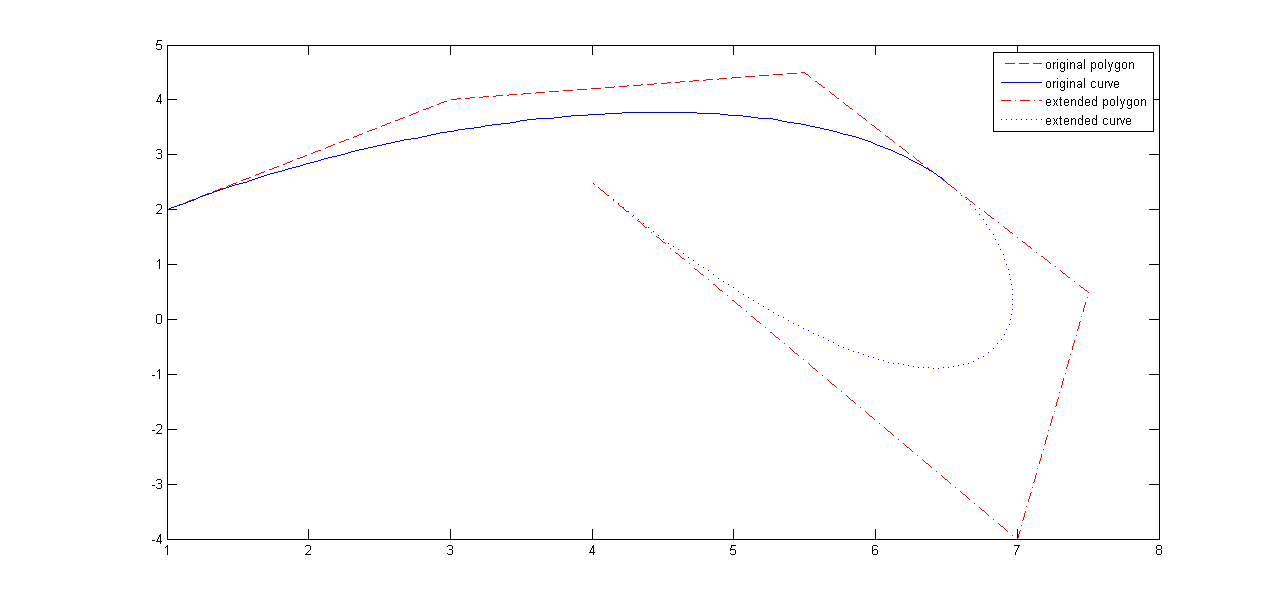
\includegraphics[width=\textwidth]{newBranch.png}
\label{fig:1}
\end{figure}

\section{Task 2}
For the visualization of the basis functions of the knot-vectors please refer to figure \ref{fig:2a} and \ref{fig:2b}! 

\begin{figure}[hbtp]
\caption{Knot-vector: $\{0, 0.25, 0.5, 0.75, 1\}$}
\centering
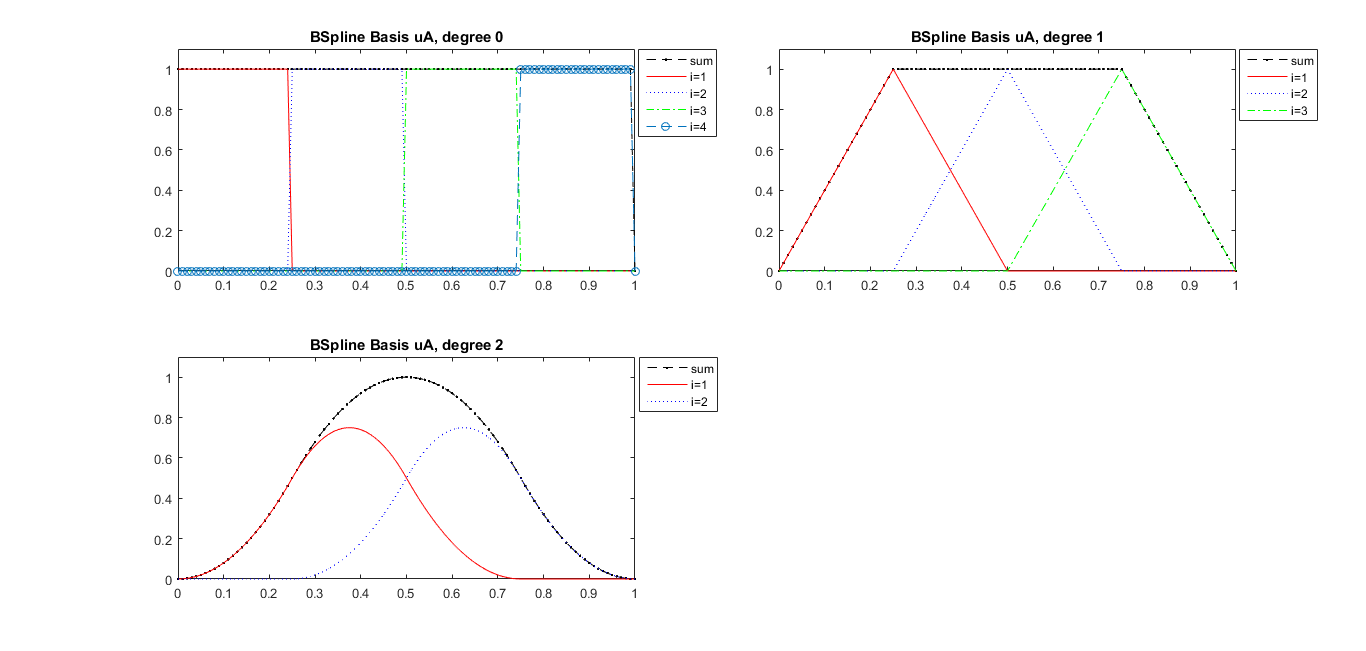
\includegraphics[width=\textwidth]{basisFunctA.png}
\label{fig:2a}
\end{figure}

\begin{figure}[hbtp]
\caption{Knot-vector: $\{0, 0, 0, 0.3, 0.5, 0.5, 0.6, 1, 1, 1\}$}
\centering
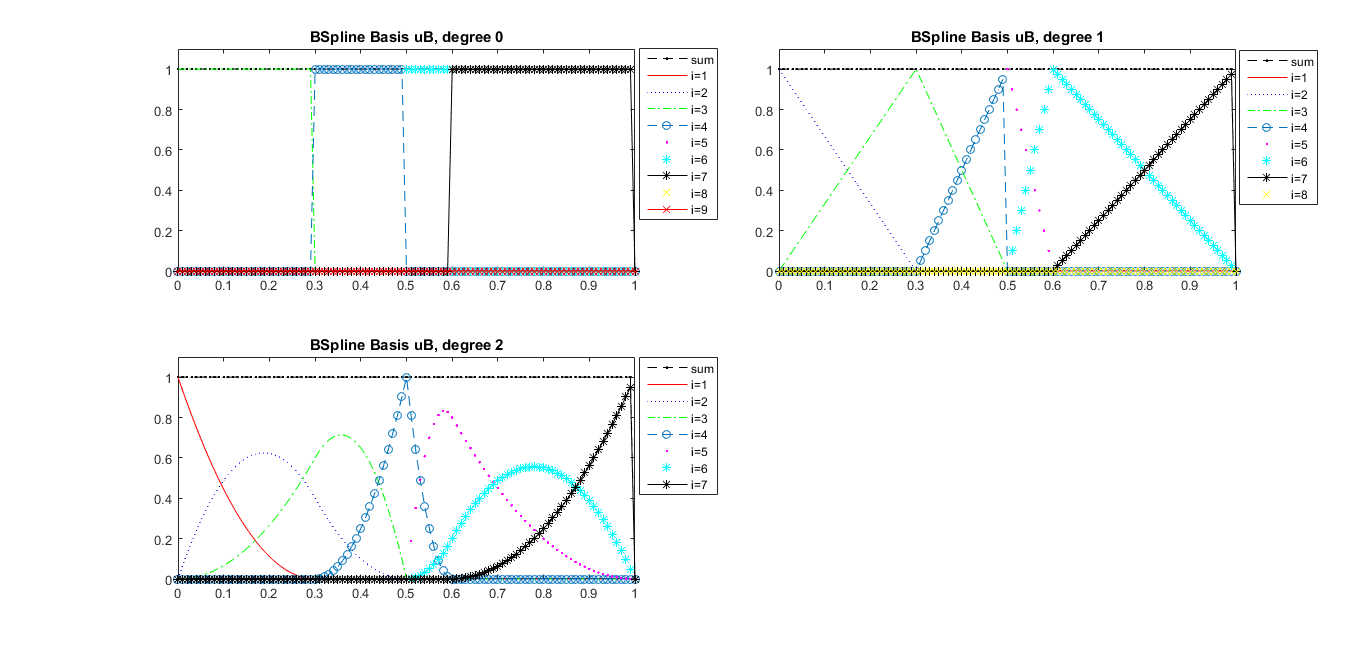
\includegraphics[width=\textwidth]{basisFunctB.png}
\label{fig:2b}
\end{figure}

\end{document}